\documentclass{report}
\usepackage[utf8]{inputenc}
\usepackage[margin=1in,includefoot]{geometry} %control margins
\usepackage[pdftex]{graphicx} %allows to import images
\usepackage{float} %allows for control of float positions
\usepackage[table,xcdraw]{xcolor}
\usepackage{multicol}
\usepackage{multirow}
\usepackage{fancyhdr}
\usepackage{parcolumns}
\pagestyle{fancy}
%\usepackage[backend=biber]{biblatex} 
%\bibliographystyle{ieeetran}

\usepackage{listings} % Required for inserting code snippets

\title{Tolerant Parsing of Models Serialised in XML/XMI}
\author{Fiifi Botchway}
\date{January 2015}

\begin{document}

\maketitle


\chapter{Introduction}
\section{Motivation for project}
\section{Report Structure}



\chapter{Literature Review}
\section{Introduction to XML}

XML(Extensible Mark up language) is a language that is used in several aspects of computing. It can be firstly used as a metalanguage(language used to describe another language) or as a method for your own markup so that one can define meaningful names for all your information items(Information identification). XML is very portable and is backed by international standards and thus is often used as a format to store information across many platforms.XML documents are widely used in many real life applications of computing such as modeling, messaging, data structure description and many more. They are a simple and versatile format that can easily be filled with errors due to its easy manipulable nature. Currently there are a few methods for identifying these errors. These errors can come in different forms, which will discuss later on in this review. In this project we are more concerned about the format and data structures that we build these XML to. In particular we are interested in the methods and algorithms used to correct and validate our XML document. This review explores different options for achieving this.

\section{XML well-formedness}
A method of XML validation and probably the most popular is validation using an XML schema. XML schemas are generally instructions and constraints that describe the structure of more than one XML document. For instance an XML document with an element "A" can only have a child called "B". This rule will be described in the XML schema (example will be shown in the XSD section later). These schemas are used to validate the XML document before the XML document is used. So in general, XML schema are used to validate data completeness, data structure and data correctness. Validation of data completeness is a check to ensure all information required by the schema is in the XML document. Validation of data structure is ensuring that structure of elements and attributes conforms to what is specified in the schema. And finally data correctness is ensuring all the rules specified by the schema are obeyed by the XML document. XML schema can be written in several languages including Document Type Definition (DTD) language which is native to XML documents and the W3C developed language XML Schema (XSD [Different from schema with a small s]) \cite{xmlschema}. To review XSD and DTD we use the Library XML document below as our reference XML.

\lstset{language=XML,
		numbers=left,
    breaklines=true,
    tabsize=2,
    basicstyle=\ttfamily}


\begin{lstlisting}[caption=Library XML Document,frame=tlrb, label={lst:libraryxml}]
<?xml version="1.0" encoding="UTF-8"?>
<Library>
	<Book name="Great Expectations">
		<Chapter name="The first chapter" pages="9">
			<Content>Once upon a time....</Content>
		</Chapter>
	</Book>
</Library>
\end{lstlisting}

\subsection{XML Schema}

The XML Schema language specifies the permitter organisation of elements in an XML document. The description of these elements goes as far as specifying the datatype of its content and its attributes. Here is a list of things that XML Schema defines.
\newline It defines:
\begin{multicols}{2}
\begin{itemize}
	\item elements that can appear in a document
	\item attributes that can appear in a document
	\item which elements are child elements
	\item the order of child elements
	\item the number of child elements
	\item whether an element is empty or can include text
	\item data types for elements and attributes
	\item default and fixed values for elements and attributes
\end{itemize} 
\end{multicols}
The XSD is therefore used as a set of rules and building blocks for a number of XML documents. Below is an example of an XSD document.
		
\begin{lstlisting}[caption=XML Library Schema,frame=tlrb]
<?xml version="1.0"?>
<xs:schema xmlns:xs="http://www.w3.org/2001/XMLSchema"
elementFormDefault="qualified">

<xs:element name="Library">
	<xs:complexType>
		<xs:sequence>
			<xs:element name="Book">
				<xs:complexType>
					<xs:attribute name="name" type="xs:string"/>
					<xs:sequence>
						<xs:element name="Chapter">
							<xs:complexType>
								<xs:attribute name="name" type="xs:string"/>
								<xs:attribute name="pages" type="xs:integer"/>
								<xs:sequence>
									<xs:element name="content" type="xs:string"/>
								</xs:sequence>
							</xs:complexType>
						</xs:element>
					</xs:sequence>
				</xs:complexType>
			</xs:element>
		</xs:sequence>
	</xs:complexType>
</xs:element>

</xs:schema>
\end{lstlisting}
Elements that contain other elements are defined as complexType elements. In the example above these are Library Book and Chapter. A simple type element is the content element in the Library XML document. Each element attribute has to be explicitly defined and this is shown on lines 10,14 and 15 in the XSD above where the data type of the attribute is also defined (xs:string).
XSD was designed to inform the validity of an XML document and from this we could produce a collection of information adhering to specific data types. Where as DTD doesnt specify what data type an attribute or element needs to be. This is part of the reason why XSD is more popular than DTD. Other reasons also include the fact that XSD supports namespaces and XML Schema is written in XML 

Now the problem with schemas is that they don't always guarantee meaningful XML documents by the end of validation especially with the use of DTD which doesn't account for data types. Therefore we could have a perfectly formed XML document that might not be what end receiver of the document might want. The way these XML documents are validated against the schemas are not standardized and therefore there isnt a single method of validation. There are many ways to do so. Therefore we will need to find an optimum way of validating these schemas against the XML documents. Validation by XML schemas also doesn't provide an automatic way of fixing the errors by itself unless assisted by some program. This is made even harder when there are multiple choices of possible solutions for an error within an XML. For example, consider the XML Schema and the XML document below.

\noindent\begin{minipage}{.45\textwidth}
\begin {lstlisting}[caption=XML Schema,frame=tlrb]
<?xml version="1.0"?>
<xs:schema xmlns:xs="http://www.w3.org/2001/XMLSchema"
elementFormDefault="qualified">

<xs:element name="A">
  <xs:complexType>
    <xs:sequence>
      <xs:element name="B">
				<xs:complexType>
					<xs:sequence>
						<xs:element name="D" type="xs:string"/>
					</xs:sequence>
				</xs:complexType>
			</xs:element>
      <xs:element name="C">
				<xs:complexType>
					<xs:sequence>
						<xs:element name="E" type="xs:string"/>
					</xs:sequence>
				</xs:complexType>
			</xs:element>
    </xs:sequence>
  </xs:complexType>
</xs:element>
\end{lstlisting}
\end{minipage}\hfill
\begin{minipage}{.45\textwidth}
\begin {lstlisting}[caption=XML Document,frame=tlrb]
<?xml version="1.0" encoding="UTF-8"?>
<A>
	<F>
		<G>This is an Example</G>
	<F>
<A>
\end{lstlisting}
\end{minipage}
Clearly the element F and G are wrong elements and are not in the schema. A possible solution is F could be replaced by B and G by D. We could also replace F with C and G with E. Both are solutions which would be accepted by the schema but the problem would be which one should be solution that is picked. For this reason we look into other methods of validation and correction as well as the software involved in these cases.

\subsection{Document Type Definition}

DTD is essentially a list of legal elements and attributes that can be used in the document. DTD is not only used for XML but can be used for HTML and any other document type in the SGML(Standard Generalized Markup Language) family. The DTD for a document is usually declared at the top of the document as \textsf{$<$!DOCTYPE html$>$} or \textsf{$<$!DOCTYPE root-element SYSTEM "filename"$>$} and refers to an external document. Below is an example of the DTD document for the Library XML document.
\begin{lstlisting}[caption=Library DTD ,frame=tlrb]
<!ELEMENT Library (Book+)>
<!ELEMENT Book (Chapter+)>
<!ATTLIST Book name CDATA #REQUIRED>
<!ELEMENT Chapter (Content)>
<!ATTLIST Chapter name CDATA #REQUIRED>
<!ATTLIST Chapter pages CDATA #REQUIRED>
<!ELEMENT Content (#PCDATA)>
\end{lstlisting}
Parents and child elements are defined in the form of brackets in DTD. For instance in line 1 of the above DTD document, Library contains Book and therefore it is a parent of Book. The "+" sign next to Book defines that the library has to contain at least one Book. Attributes in  DTD are defined in the format \textsf{<!ATTLIST element-name attribute-name attribute-type attribute-value>} where for the last parameter, we can specify that a value is required instead of specifying a default value. As we can see from the example above data types are never defined.

\subsection{Ecore a simpler solution to xml schema }

Ecore is model description language tool part of the Eclipse Modeling Framework \cite{eclipsemodelingf} and can be used as a simpler solution to xml schema due to its easy to understand nature. The concept of using models to describe a data structure seems to be easier to understand than learning a syntax for a schema. This is because using models can easily give the user a visual representation of the structure of the document in the case where a model is used as a schema. This has been the motivation for research in developing methods of converting XML Schema to Ecore models which can be seen in \cite{xmlschemecore}. A more detailed and updated version of how this can be done can also be found in \cite{budinsky2004eclipse}. Ecore is a collection of interfaces and components that collectively that can be used to create a model. Figure \ref{fig:ecorehierarchy} shows the components involved in the Ecore packages.

\begin{figure}[H]
\centering
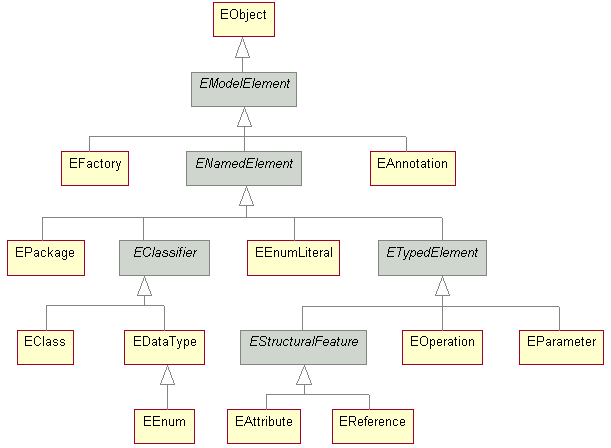
\includegraphics[width=3in]{EcoreHierarchy}%
\caption{Ecore components hierarchy obtain from \cite{ecorehierarchy}}%
\label{fig:ecorehierarchy}%
\end{figure}

Some of these components are similar to the ones found in UML. Thus we can create class diagrams to illustrate structures of schema. For example to create a schema for library XML document in \ref{lst:libraryxml} we can create the following emf file that can generate an ecore model using the tools in the Eclipse IDE.
figure \ref{fig:libraryemf} shows an emf file of the library file. This syntax is much simpler than writing a schema in XSD. The equivalent class diagram can be shown in figure \ref{fig:libraryclass}. 

\begin{multicols}{2}
\begin{figure}[H]
\centering
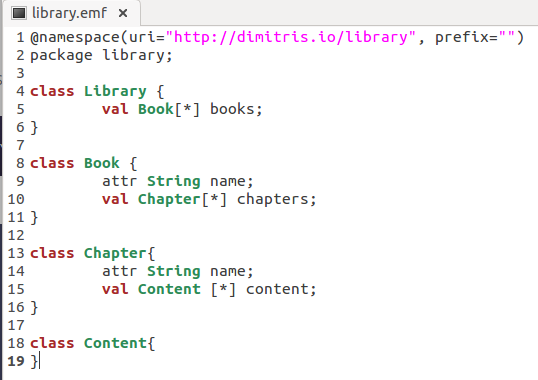
\includegraphics[width=3in]{libraryemf}%
\caption{Library Metamodel in emf}%
\label{fig:libraryemf}%
\end{figure}
\begin{figure}[H]
\centering
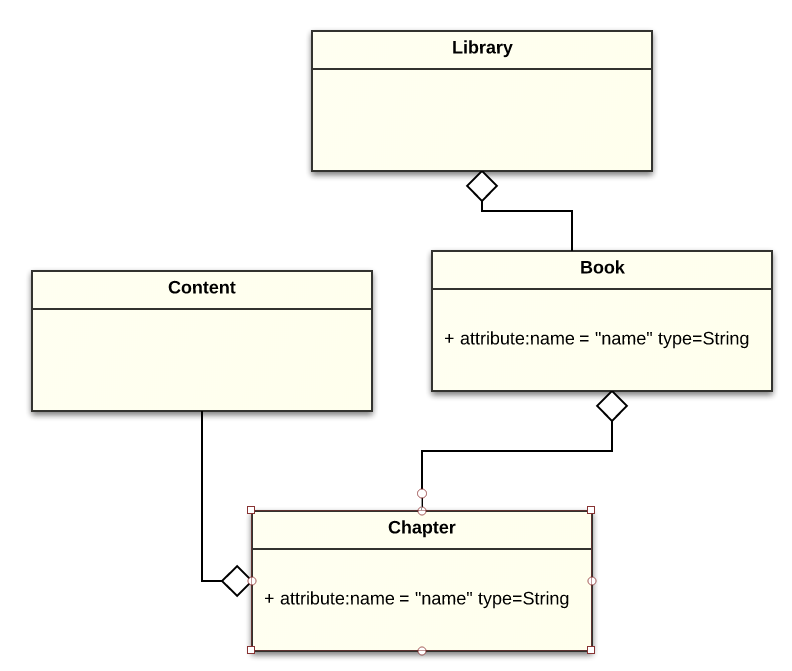
\includegraphics[width=3in]{libraryclass}%
\caption{Library metamodel in Ecore's graphical notation}%
\label{fig:libraryclass}%
\end{figure}
\end{multicols}

With the aid of eclipse, we can simplify the creation of schema for XML to creating classes with attributes and children. The tools in eclipse are sufficient and powerful enough to convert these simple class constructions into ecore files which can be a powerful tool to use in validation.

\section{XML Correction Methods}
\subsection{XMLVC}

Guan Ying and his colleagues at NanKai University in China propose a model that attempts to achieve XML Correction. The model is called the XMLVC (XML Validation and Correction) \cite{ying2012xmlvc}. The model is based on a set of algorithms for incremental validation and correction and also uses DataGuide \cite{goldman1997dataguides} which is a validation algorithm which shortens the cost time when validating a whole document. The concept of the algorithms used for incremental validation is that after full validation run by DataGuide, they get which nodes(Elements in the XML document) are at fault. From that node they get a subtree of the full XML document with the faulty node as the root. This then is either repaired deleted or replaced using the schema and a correction algorithm. This algorithm is shown in figure \ref{fig:xmlvccorrectionalgo}. It replaces nodes that are not in the schema with the next similar child of the parent node, and for other errors such as occurences of nodes and its attributes, it only gives back a warning for the user to change manually. DataGuide then runs on that subtree before it is put back into the main document. DataGuide achieves efficiency by shortening a tree so that there aren't any duplicate branches before validation. Each node in the tree has a corresponding node\_model \cite{ying2012xmlvc} which contains schema information about the node (nodetag, max occurrences, min occurrences, attributes, children, type etc.). This is the basis used in the validation.

\begin{figure}[H]
\centering
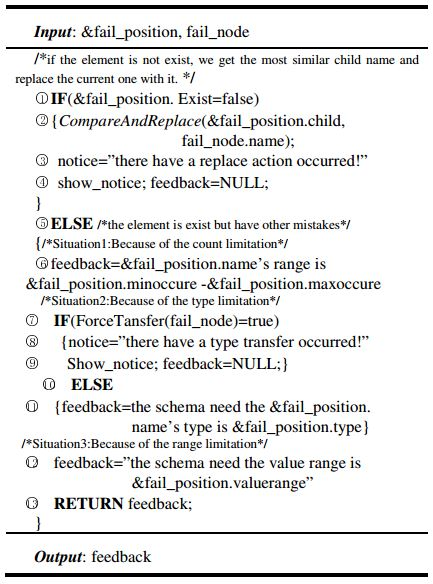
\includegraphics[width=3in]{XMLVC-correction-algorithm}%
\caption{Correction algorithm from the XMLVC paper \cite{ying2012xmlvc}}%
\label{fig:xmlvccorrectionalgo}%
\end{figure}

%\subsubsection{Tree-To-Tree Correction for Document Trees}
%\subsubsection{XML Correction with XML Query Analysis}

Although the paper on the XMLVC model might be a good solution to validation, it and other papers regarding validation and correction of XML \cite{barnard1995tree} \cite{starka2011xml}, are more concerned about efficiency than correction. There can sometimes be very ambiguous mistakes made in XML that most of these paper's solutions might miss. For example, the solution in the "Analysis with Analyzer" paper has a method and algorithm that could come up with several possible solutions for an incorrect XML and evidently pick a solution according to schema but not what the user intended. For this, we looked into the paper about similarity flooding. 

\subsection{Incremental String Correction}
There has been some research by Ahmed Cheriat et. al\cite{cheriat2005incremental} on the topic of XML correction with respect to regular grammars. The concept of this is based on incremental string-to-string correction. This is correcting a single modified string based on its previous form and the set of updates performed on the string. For example we have a string \textsf{A} and with a set of update functions (delete add or replace words in the string) we get the String \textsf{B}. We have a regular grammar grammar rules that the output string \textsf{B} has to conform to and if not we detect an error and try to correct it. The paper \cite{cheriat2005incremental} tries to correct this string by considering the set of updates performed to the word as well as the edit distance between \textsf{A} and \textsf{B} and the set of viable candidates(SC\textit{andid}). SC\textit{andid} is a set of solution conforming to the regular grammar that the algorithm produces in which the users has to choose from. A finite state automaton is used to produce these solutions. To briefly explain this, lets consider an instance mention in \cite{cheriat2005incremental} where we have a grammar $E = (aba + bab)*$, A valid word $A = bab$, a sequence of updates performed on A $S = (insert(a,1),replace(a,2))$ (where the second parameter in each update is the index of where the action should be performed using 0 as the first index), and an invalid word $B = baaa$. Since there are only two actions performed on the original word we can only produce possible candidates $C$ that are of edit distance less than or equal to two. This is the threshold $th = 2$. Given this, the algorithm runs these values through a finite automaton where the accepting state is a word C that is accepted by the grammar where the edit distance between $A$ and $C$ is $\leq th$ and the edit distance between $B$ and $C$ is $\leq th$. We also have the transition functions as possible edits to the solution word $C$. In the initial state of this automaton, $C$ is a partial valid candidate word for example it could be $aba$. Each time the automaton finds a solution $C$ it adds it to the $SC\textit{andid}$ list. More about the automaton can be found in \cite{cheriat2005incremental}. After the automaton is run we get a set of solutions  $SC\textit{andid} = ((aba,(2,2)),(bab,(0,2)))$. The numbers in the brackets next to each solution represents the edit distance between $A$ and $B$ respectively. From this, the user chooses their intended solution and another algorithm is in place \cite{cheriat2005incremental} to show which update functions need to performed to get to that solution. The paper suggests that these technique can easily be applied to XML documents by thinking of the string as tree whose depth is 1 and whose leaves are the element of the string. So for example in the library xml example mention previously, we can cut the xml at depth 1 therefore cutting off at the book element where the book element is one of the leaves. 

This incremental string correction technique is very useful in the case of correcting XML documents that have been updated and were initially valid but becomes very difficult for instances where the initial XML document created is invalid and needs to be corrected. This is because we cant compare a solution to a previous state of the document. 

 
\subsection{Similarity Flooding}

Similarity of graphs and elements was what the previously mentioned papers were lacking. Sergey Melnik \textit{et. al's} paper \cite{melnik2002similarity} on similarity flooding proposes a way of graph matching which can be applied to schema matching. The paper describes a matching algorithm that takes an input of two graphs and based on a fixpoint computation, outputs a mapping between corresponding nodes. During the algorithm, all possible pairings between the two input graphs are made. The algorithm then attempts to form connections between these pairing to create one graph of pairings and connections. The connections are formed by a condition that to connect a pair (A,B) to (A',B') , there exist a connection from A to A' in one of the input graphs and there exist a connection B to B' in the other input graph. If this condition is not met, the pair is discarded and not added to the paired graph. The algorithm then evaluates the graph using fixpoint computation which takes into consideration the edges between nodes and how many connections each node has. The result is a similarity score of the pairings to show which pairings are the strongest. This can be illustrated in the picture below.

\begin{figure}[H]
\centering
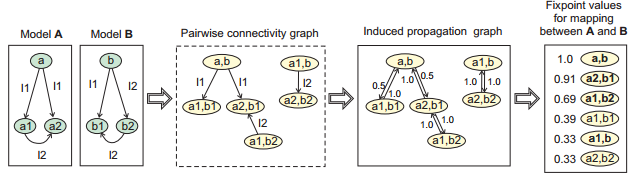
\includegraphics[width=6in]{similarityfloodinggraph.png}%
\caption{Process of graph matching and fixpoint computation from Melnik's paper \cite{melnik2002similarity}}%
\label{fig:simfloodgraph}%
\end{figure}

\section{XML Correction Software}
\subsection{Intelligent Correction and Validation Tool for XML}
This is a program in the Perl programming language developed by Abhishek Shivadas \cite{shivadas2001intelligent} at the University of Kansas as part of his masters degree. The program focuses on mutated schema and how validation and correction of XML documents can be achieved using these newly formed schemas. In the paper on this program \cite{shivadas2001intelligent}, he identifies the major changes to schema that inevitably make an XML document invalid. These changes are the order change of elements, renaming of element tags, adding/deleting tags, and changing tag/attribute values. He designs the program to identify these changes, suggest XML changes  and perform these changes when prompted by the user. The program does all of this in three phases. The first phase is the translation  of a given schema to a format that will be process by the program. This process is repeated every time the schema is changed. The second phase is when the XML document is validated against the schema and changes are suggested. After user input, the third phase is exucuted which performs the user desired changes on the XML document. 

We will firstly look at the first phase in detail. This part mainly involves a perl module which is responsible for taking an XML Schema as an input and breaking down its structure into a comma delimited format(also known as a csv file). With this, the data can be sorted as a table. This table is then used for validation. The table created contains each element in the XML Schema and its properties. These are the columns in the table. The properties of each element are the path(order of element), its required sub element(s), the legal values the element must contain(this could be null), the minimum and maximum number of times the element can occur, the order in which each sub element can occur, the valid attributes of the elements, and the last property is a Boolean which determines whether the set legal values the element must contain should be in the attributes or in its text. Below is an example of how the XML Library Schema mentioned previously will be translated into a table. 


\begin{table}[h]
\begin{tabular}{|l|l|l|l|l|l|l|l|}
\hline
\multirow{2}{*}{\textbf{Path}} & \multirow{2}{*}{\textbf{Required Tag}} & \multirow{2}{*}{\textbf{\begin{tabular}[c]{@{}l@{}}Enume-\\ ration\end{tabular}}} & \multirow{2}{*}{\textbf{Min}} & \multirow{2}{*}{\textbf{Max}} & \multirow{2}{*}{\textbf{Sequence}} & \multirow{2}{*}{\textbf{Attributes}}                 & \multirow{2}{*}{\textbf{\begin{tabular}[c]{@{}l@{}}Bool-\\ ean\end{tabular}}} \\
                               &                                        &                                                                                   &                               &                               &                                    &                                                      &                                                                               \\ \hline
/Library                       & Book                                   & -                                                                                 & 1                             & 1                             & Book                               & -                                                    & f                                                                             \\ \hline
/Library/Book                  & Chapter                                & -                                                                                 & 1                             & U                             & Chapter                            & name                                                 & f                                                                             \\ \hline
/Library/Book/Chapter          & Content                                & -                                                                                 & 1                             & U                             & Content                            & \begin{tabular}[c]{@{}l@{}}name\\ pages\end{tabular} & f                                                                             \\ \hline
/Library/Book/Chapter/Content  & -                                      & -                                                                                 & 1                             & U                             & -                                  & -                                                    & f                                                                             \\ \hline
\end{tabular}
\end{table}

The next phase which is the core aspect of the program is the validation and correction suggestions of the XML document. This part of the program is activated by the user uploading an XML document. The program then starts with the root node and validates it against the table first row. In then goes down the tree, exploring each sub element validating and looking for inconsistencies. This is done recursively until the leaf nodes are reached. When inconsistencies are found, the program analyses these inconsistencies to find solutions. All solutions found through out this process are store in a file called the control file which is later shown to the user to select which solutions to implement.

The process of validating the XML document is done by seven modules in the program. The architecture of this can be seen in figure \ref{fig:phase2arch} below
%%%%%%%%%%%%%%%%%%%%%%%%%%%%%%%%%%%%%%%%%%%%%%%%%%%%%%%%%%%%%%%%%%%%
\begin{figure}[H]
\centering
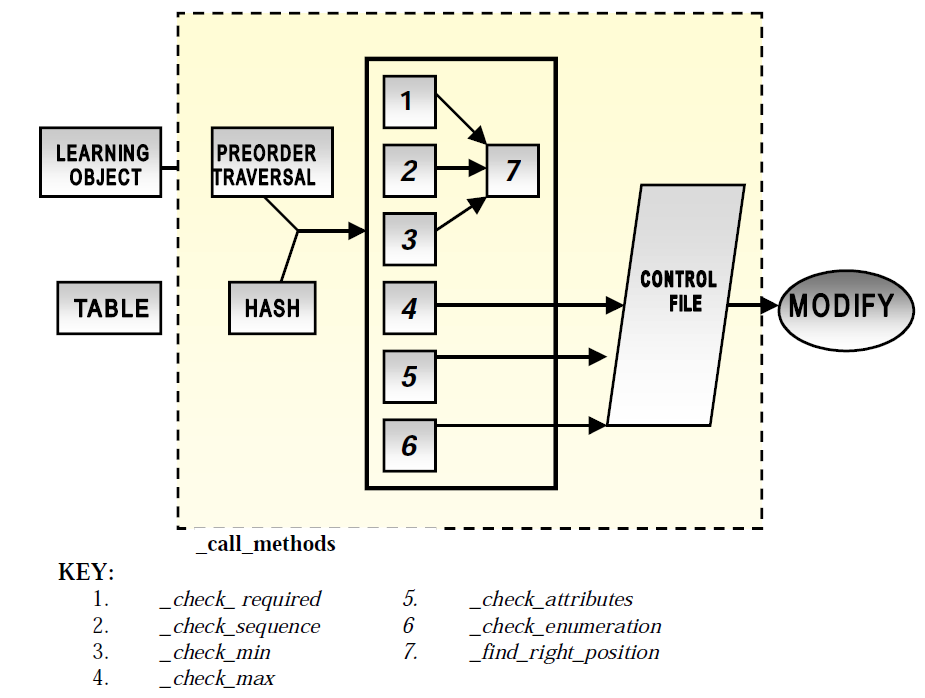
\includegraphics[width=4in]{phase2arch.png}%
\caption{Phase 2 software architecture from \cite{shivadas2001intelligent}}%
\label{fig:phase2arch}%
\end{figure}
%%%%%%%%%%%%%%%%%%%%%%%%%%%%%%%%%%%%%%%%%%%%%%%%%%%%%%%%%%%%%%%%%%%%%%%

From the above diagram we can see that this part of the program takes two inputs, the XML document(Learning Object) and the Schema Table. It then traverses through the document and table implementing all the modules 1-7. Thus outputting a control file that determines what needs to be changed.
The modules are essentially subroutines that check that the properties of each element mentioned previously in the schema table have been satisfied. In the instance where a property is not satisfied, the module return an array of elements which a set of "primitive actions" will be performed on. In the paper \cite{shivadas2001intelligent}, Shivadas describes these primitive actions as adding, deleting, moving, renaming, and modifying. The primitive action performed on each element will be determined by which module the output array comes from. For example in the "check{\_}required" module, the algorithm gets all the required of the tag from the table and traverses through the list to see if any required elements are missing. It then stores all the missing elements in an array and because this array came from the "check{\_}required" module, an add primitive action will be performed on the elements. Further details of this can be found in \cite{shivadas2001intelligent}.The 7th module is used for the first three modules because it is called whenever an element needs to be inserted or modified. The module calculates and stores the position in which the action needs to be performed. Details of the algorithm used is described in \cite{shivadas2001intelligent}. The other modules are pretty self explanatory in what their functions are by looking at their names.

The final phase of this program is implementing the approved changes of the user in the XML document. This phase is only initiated if after validating there are suggested changes that need to be made. Like the previous phase of the program, this script also uses a modular architecture to implement the corrections. This is shown in figure \ref{fig:phase3arch} below.

%%%%%%%%%%%%%%%%%%%%%%%%%%%%%%%%%%%%%%%%%%%%%%%%%%
\begin{figure}[H]
\centering
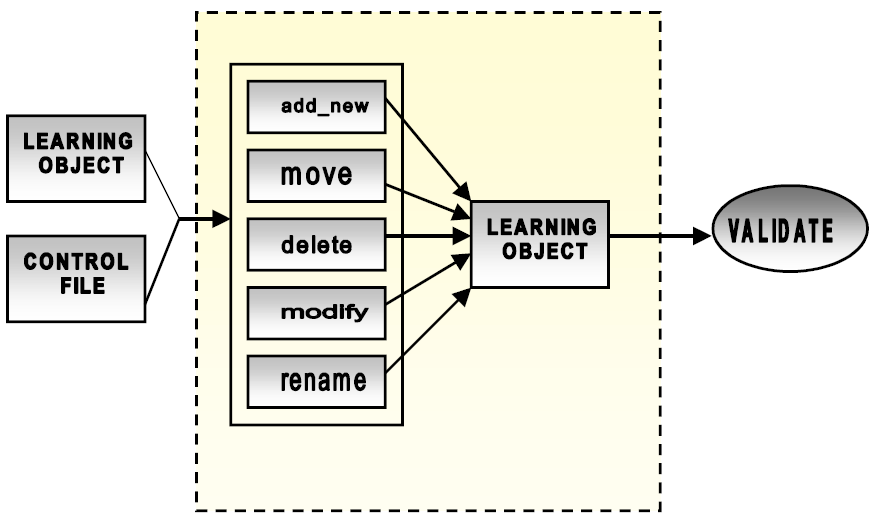
\includegraphics[width=4in]{phase3arch.png}%
\caption{Phase 3 software architecture from \cite{shivadas2001intelligent}}%
\label{fig:phase3arch}%
\end{figure}
%%%%%%%%%%%%%%%%%%%%%%%%%%%%%%%%%%%%%%%%%%%%%%%%%%

From this we can see that the modules that are used on the XML document are the the primitive actions defined previously. This part of the program goes through each entry in the control file and execute a corresponding module on the XML document. After each entry has been traversed, the output XML document is then validated again. Each of the modules are pretty straight forward apart from the move module. 
The move module could perform four types of move operations. The first is moving a single element before or after another. The second is moving a single element before or after a number of elements. The third is moving a number of elements before or after a single element. Finally the last is moving a number of element before or after another set of elements.

The good thing about this software is that the design of its architecture permits the program to run fast.  This is possible by the use of hash tables in when accessing the schema as we have an access time of \textit{O}(1). 

The bad is that since the program has no aspect of similarity when comparing elements to schema, it will have difficulty producing valid solutions to rename tags in the schema. For instance with the library XML schema, if we renamed the "Book" element to "Journal" but with the same attributes and properties(children and parents), the program wont suggest a rename but instead a delete or add solution. The program is also not very good at adapting to schema changes where elements are moved from within its local parent to another parent. For example if we modified the XML Library schema to have "Department" as a child of Library and then "Category" as a child of Department, and put the "Book" element and its children as a child of "Category", the program wont be able to move "Book" and its children to the appropriate place given that "Book" is placed at the same level as Department(as a child of library) in the XML document. The program will instead attempt to re-create the structure of the schema by deleting and adding elements instead of performing a move operation on the misplaced elements. 

\chapter {Problem Analysis}
\section{Analysis}
There is not much literature on XML Correction methods and less so software that implement these methods and therefore reinforces the need for such technologies. 
\section {Potential further work}
\subsection{Trie structure and algorithm}
Tries are dynamic data structures which are usually used for looking up words and elements. They contain a group of nodes which are grouped together in a specific way. They are mostly used for looking up words from a dictionary where the trie is the dictionary. Tries, although not specifically used for XML correction, can be deployed within this area. To explain how these works we will use figures \ref{fig:triestep1}, \ref{fig:triestep2} and \ref{fig:triestep3}to illustrate the process of using Tries. Let us firstly assume we want to create a small dictionary containing the words "ACE" "ACES" "ACER" "ACT" "ACTOR". Notice how some of these words are prefixes of the other. In figure \ref{fig:triestep1} we start building our dictionary. The mark the final letter in our word with an identifier. In this case it is "E" for the word "ACE". We can then add "R" and "S" at the end of "E" without creating a separate trie for this as shown in figure \ref{fig:triestep2}. In figure \ref{fig:triestep3} we complete the trie which can now hold 5 words with only 8 characters instead of 19. Now we can check the Words that we defined in the begin against the trie. For example we can check that "ACE" is a word by starting from A and working our way down. If we tried inputing the word "ACTO" we will quickly realise that this is not a word and reject it as "O" doesn't have an identifier


\begin{multicols}{3}
\begin{figure}[H]
\centering
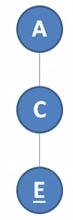
\includegraphics[width=0.5in]{Triestep1}
\caption{Trie data structure 1 from \cite{youtubetrie}}
\label{fig:triestep1}
\end{figure}
\begin{figure}[H]
\centering
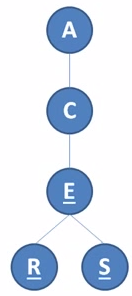
\includegraphics[width=1in]{Triestep2}
\caption{Trie data structure 2 from \cite{youtubetrie}}
\label{fig:triestep2}
\end{figure}
\begin{figure}[H]
\centering
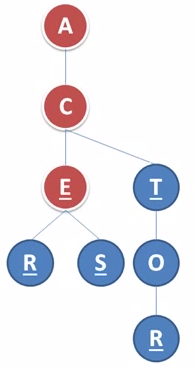
\includegraphics[width=1in]{Triestep3}
\caption{Trie data structure 3 from \cite{youtubetrie}}
\label{fig:triestep3}
\end{figure}
\end{multicols}

The trie algorithms that are used with these data structures are used to find words that prefix or are contained in words in the dictionary
From this type of data structure we could extend the application to validation in XML by having the nodes contain possible elements and storing information such as limits and containment conditions in the edges connecting these nodes.Therefore we this technique we could have both syntax checking as well as checking the XML for well formedness. We could even extend it even more and attempt to use it in automatic correction. We could do this by traversing through the nodes and when the end node reached is not an identifier we could calculate a cost funtion that will determine the all surrounding identifiers and the amount of nodes it would take to get to them(the cost). We would then chose the shortest path and consider that a solution.  
Searching using trie structures is often fast than other data structures and therefore if implemented as a validation technique can be very efficient

\chapter{Requirements}
This section will cover the Stakeholders involved with this project, the requirements covered and some use cases to illustrate scenarios in when this project can be applied.

\section{Stakeholders}
The stakeholders are parties that have interest or stake in this application. Knowing who the stakeholders aids in capturing each essential requirements and justifies why each requirement is needed. Thus we can trace each requirement back to the needs of a stakeholder in this project. A list of these stakeholders can be found below.

\begin{itemize}
\item \textbf{End-Users}- These are generic software developers that use XML documents in their own projects and will need to verify and correct these XML documents.
\item \textbf{Software Extenders} -  These are software developers that are interested in extending the capabilities of this application.
\item \textbf{Project Developer}
\item \textbf{Project Supervisor}
\end{itemize}

\chapter{Design}
\chapter{Implementation}
\chapter{Testing}
\chapter{Evaluation}
\chapter{Discussion/Conclusion}
\section{Security Aspect}
\chapter{Further Work}


\bibliographystyle{IEEEtran}
\bibliography{ReportBib}

\end{document}
